\chaptertitle{4}{投资必备的基础知识}
\setcounter{figure}{0}\setcounter{table}{0}
我们已经明白了定投的含义。定投就是定期把人力资产转换为可以产生现金流的金融资产。当这些资产产生的现金流可以满足我们的日常生活支出，我们就实现了财务自由。这也是定投的目的。

不过，同样是定投，定投不同类型的资产，最后积累财富的效果也会有比较大的差别。

那我们普通投资者在日常生活中，有哪些可以定投的金融资产呢？按照性质，通常可以分为货币、债券、股票三类。

我们可以直接投资这些资产，例如开通股票账户，投资股票，或者直接去货币市场投资。不过不同的投资品种，交易门槛有很大差别。例如，货币市场，可能需要500万元才能进入；股票里的贵州茅台，交易一次就需要七八万元；部分债券，门槛也是比较高的。

所以普通投资者，通常是通过一些间接的金融产品来投资这三类工具。而提供这些工具的，通常是银行、基金公司等机构。

像我们熟悉的银行理财产品、股票基金，都算是间接投资工具。这些间接投资工具的门槛并不高，像大部分基金只需几十元就可以投资。银行理财可能门槛高一些，但也是普通投资者可以接受的。

我们来分别了解一下。

\subsection{银行系理财工具都有哪些}
\subsubsection{银行储蓄，开启理财的第一步}

我们用得最多的金融工具，当属银行的金融产品了。几乎每个人都有银行卡，也都用过银行的储蓄产品。

在二十世纪六七十年代，我国的金融市场还不发达，大家并没有投资理财的意识。每个月发到手的钱，很多人习惯用现金的方式存着，甚至会仔细包好，放在隐蔽的地方，需要用的时候再取。

直到银行开始兴起，大家才意识到，原来手里的现金还可以存到银行，不仅更加安全保险，还可以获得利息，愿意接受新事物的人开始尝试把钱存到银行。到九十年代，银行已经被大多数人所接受，很多人把积蓄变成储蓄放在银行里。不过习惯的力量还是非常强大的，一部分人仍然无法接受银行这一新事物，坚持把现金存在家里。所以时不时能看到新闻说某老人家埋在自家后院的现金被老鼠啃食。

后来大家就有了将钱存银行的意识了。因为钱存在银行，还能让钱增加一点。

对任何一家银行来说，储蓄都是银行的根本。银行业也有一句话，“存款立行，贷款兴行”。如何揽储，是银行发展的重中之重。

银行的储蓄产品主要分为活期和定期。其实我们开通银行卡之后，卡里只要有钱，就会自动享受活期储蓄的收益，而定期是需要我们手动开通的。

在定期储蓄中，就有一类，个人零存整取业务，是指储户跟银行签订零存整取协议，储户自己设定一个金额，每个月定期存入一笔资金。中间如果有遗漏，下个月可以补上。如果连续两个月没有补，就被视为违约。零存整取协议就自动解除。

这种零存整取协议，就是一份非常标准的定投计划，只不过是围绕银行产品来的。

零存整取业务，也有一些衍生的品种。教育储蓄就是一个典型，其实它也是以银行储蓄为核心，但是在执行的时候带入了一个具体的应用场景，即为孩子的教育做一个长期的定投。

那这种银行的零存整取业务，收益高吗？

其实银行储蓄无论是活期还是定期，主要是安全稳定，几乎不会亏损，所以收益不会太高。

以2019年2月1日，国内央行基准利率为例。

{\kaishu 活期储蓄，利率为0.35\%。}

{\kaishu 3个月定期存款，利率为1.1\%。}

{\kaishu 6个月定期存款，利率为1.3\%。}

{\kaishu 1年定期存款，利率为1.5\%。}

{\kaishu 3年定期存款，利率为2.75\%。}

不同银行可能会在这个基础上有所浮动，例如中小银行的定期存款利率通常会比基准利率高一些，但也高得有限。

虽然收益率不高，但银行储蓄的定投，是许多投资者做的第一笔定投。甚至许多人在上学的时候，就已经开始做基于储蓄的定投了。虽然收益率低，但也是一个完整的定投策略。

\subsubsection{长远来看，把钱存在银行不划算}

长远来看，储蓄无法帮助一个家庭的资产得到较多增值。我们看一下日本储蓄的案例。

日本跟国内有一个非常大的区别，即日本市场是负利率的。

这个负利率并不是说个人存在银行的钱一点儿利息都没有，而是银行机构存在国家银行的一部分资金是负利率的，以此推进银行多放贷、多做业务。刺激经济，是这个政策的初衷。

个人在日本将钱存在银行，还是正利率的。

不过就算有利率，也没多少钱。2015年，日本活期存款利率从0.02\%降到了0.001\%，几乎是没有收益的。也就是，存100万元，一年利息只有10元。

所以在日本，存款是很不划算的事情，几乎跟持有现金没有区别。

中国目前还没到这一步。但是从长期看，储蓄的利率确实是会逐渐降低的。所以仅仅是储蓄，对家庭来说是远远不够的。

不过遗憾的是，国内确实有相当数量的家庭，每个月获得的收入，就是放在银行的活期储蓄里。相当于按月定投活期储蓄。这是一个收益很低的定投。对这些家庭来说，还是要尽早改变观念。

\subsubsection{银行理财产品的优缺点}

除了储蓄产品，银行理财产品也是一类经常接触到的投资品种。

银行理财产品看起来跟定期储蓄很相似，不过也有几个不同的特点：

（1）银行理财产品的门槛比较高。

储蓄类通常门槛比较低，而银行理财产品的门槛要高一些。早期银行理财产品的门槛普遍是5万元。后来出台了新规，部分银行理财产品的门槛降到1万元。

（2）银行理财产品在特殊时点收益高。

银行理财产品在部分特殊时间点，收益会高一些。例如季末、年中、年末，这些考核的时点。

在这些时点，一方面市场本身资金面可能会紧张一些，另一方面银行也有自己的考核要求，员工也有业务量的要求。所以在这些时点银行理财产品的收益率会比较高，以此来吸引客户投资。

（3）小银行的收益率一般比大银行高。

这个很好理解。规模越大的银行大家越信赖，越不愁客户，获客成本低。小银行如果不提高理财产品的收益率，就很难吸引客户了。

具体哪家银行的收益率高不好确定，有的地方某家银行比较强势，换一个地方就比较弱势，没有统一的排名。一般银行的收益率从低到高可按：国有银行<商业银行<城商行、农商行<信用社，不过风险也是越来越高。

到城商行级别就有一定风险了。城商行往往跟当地机关、国有企业联系紧密，如果这些企业出现问题，城商行还是挺有压力的。不过大城市的城商行，如北京银行、上海银行，风险相对较小。如果本地的城商行不太靠谱，还是从国有银行和商业银行中选择。

大多数人不可能亲自去每家银行了解，可以在网上搜索每家银行最新的存款利率表。一般存款利率高的银行，理财产品的收益率也高。

（4）即使同样的产品，客户在银行的级别不同，获得的收益率也不同。

很多银行会给客户评级，高等级客户可以享受更好的产品，得到更多的信息。

银行内部也会根据客户的资产量，来划分不同的客户级别。高资产量的客户，接触到的理财产品的收益率通常也会更高一些。

不同银行的客户等级升级难度不同，甚至同一家银行不同网点也不同。之前螺丝钉有一张普通卡，某个网点要求存入资金才能升级，而另一个网点没有任何要求就帮我升级了，所以可以多试试。

升级为高等级客户，银行会提供收益率更高的产品、更多的信息、更好的服务。除了收益率高，还会赠送洗车、机场贵宾厅、饭店优惠、航空里程等服务。不过这不是无条件的，一般会要求客户存入一定金额的资金，保留一定的时间。

有的朋友会把钱存在多家银行，其实不如集中优势兵力逐个击破，在一家银行把等级提升起来，这样可以获取更多的权益。

（5）一般期限越长，收益率越高。

银行理财产品是一个资产大类，既有类似货币基金这样随取随用的品种，也有类似定期储蓄这样半年期、一年期的品种。目前，银行销售的理财产品还是主要集中在一年期以下。

随时申购随时赎回的品种，流动性好，适合作为现金替代品，当然收益率也最低。

另外还有以一周、一月、一季度、半年、一年等作为周期的理财产品。随着期限的增长，收益率也会增加。

例如，有10万元大约4个月后会用到，但不知道确切的日子。我们就可以先购买3个月期限的理财产品，再购买1个月期限的理财产品，最后换成7天期限的理财产品，临近使用的时候换成货币基金。这样可以获取最高的收益。

（6）其他方面的优惠。

其他的一些优惠主要是跟银行的其他产品构成的。

现在银行都讲联动营销，意思就是多个产品一起推广。例如对办理了住房贷款的客户，银行往往再会推荐装修贷这样的消费贷款。

理财产品也是一样。如果在一家银行有大额理财产品，之后在同一家银行办理大额信用卡、银行贷款等都会更容易一些。很多银行卡有不错的活动或优惠，贷款如果利率有优惠也是很不错的。

不过从整体来看，银行理财产品主要投资的是债券类品种，本身的长期收益率在4\%～6\%，比银行储蓄的收益率高，但也不会高太多。

银行储蓄和银行理财产品，是我们最常用的银行系理财工具。大部分朋友可能没有买过基金和股票，但是银行储蓄和理财产品应该都接触过。

不过银行储蓄和理财产品都是主要投资债券类品种，安全性不错，但长期收益是比较低的，单靠银行储蓄和理财产品，比较难跑赢通货膨胀。

\subsection{基金，最适合普通投资者的工具}
除了银行的金融工具，基金也是我们经常接触到的投资工具。

基金，是一种间接的投资工具。我们把钱交给基金公司，基金公司拿着这些钱，去投资各种资产。如果基金赚了钱，我们也就赚了钱；如果基金亏损，我们也要承担亏损。

简单理解，基金就是一个篮子，里面可以按照预先设定好的规则，装入各种各样资产。这样做的好处是，把一篮子资产分割成若干小份，一小份才几元钱，用较少的资金就可以投资了。这样一来，原来普通人买不起的资产，现在可以通过购买基金的方式投资了。

基金是一类非常庞大的资产，有各种各样不同的形式，最常见的有公募基金、私募基金，养老、社保基金，以及其他的，比如国家主权基金等。这么多的基金种类中，我们普通投资者能投资的、平常接触最多的，就是公募基金了。本书所提到的基金，指的也是公募基金。

\subsubsection{基金投资的好处}

为什么说基金最适合普通投资者呢？主要是基金有如下三大好处。

第一个好处，每一只基金都有专门的基金经理来为我们打理，他们可以帮我们投资一些我们不熟悉的品种，另外，基金也降低我们的投资门槛。

像国内股票有几千只，大多数投资者是不了解这些股票背后的公司的，而基金经理可以帮我们去投资这些股票。

另外，像股票市场和债券市场，进入的资金门槛不同。如果是货币市场这类品种，投资者需要500万元以上的资金才能开始配置，很明显超过了普通人的承受范围。但是不同类型的基金品种，投资门槛差别不大，基本都是几十元起。交易的规则也差不多，大大降低了普通投资者的投资门槛。

第二个好处，基金可以很方便地分散风险。我们都知道，不要把鸡蛋放在同一个篮子里。理论上讲，持有多种不同的资产，可以有效地分散风险，但是这需要我们去选择投资十几只，甚至几十只不同的投资品种才能达到。这对于普通投资者来说还是比较困难的。而基金一般都会投资几十只不同的品种，大大减少了只投资单一品种的风险。

第三个好处，投资基金不需要频繁操作，比较省心省力。大多数投资者都想通过投资实现资产增值，但是我们一般都有自己的正常工作，没法像专业投资者那样拿出大量的时间和精力来专职投资。不过，无论哪种基金，都有基金经理负责维护。我们只需要选对品种，剩下的，基金经理会帮我们完成，比较省心省力。

选择基金进行投资，是很适合我们普通投资者的。因为普通投资者不具备专业投资者的研究能力，也没有时间去做太深入的研究。通过基金去投资，可以节约很多时间成本，也避免了很多风险。所以在全世界范围内，基金都是普通投资者最常用的一类投资工具。

我们通过定投基金，可以自由地搭配出我们想要的投资效果，满足家庭所需。

不过国内的基金总数量可是非常庞大的，加起来有5000多只。这么多的基金，我们普通投资者是无法一一掌握的。

那么，我们该如何了解基金呢？

\subsubsection{基金都有哪些分类}

基金是一个非常庞杂的资产类别，我们先来谈谈基金的分类。基金有很多种分类的方式。

（1）按照投资方向，基金可以分为：股票基金、债券基金、混合基金、货币基金。

我们可以把基金想象成一个包子，它可以装入各种馅料。

{\kaishu 肉包子：股票基金，基金里装的80\%以上是股票。}

{\kaishu 素包子：债券基金，基金里装的80\%以上是债券。}

{\kaishu 什锦包子：混合基金，股票债券都有，比例比较灵活。}

{\kaishu 糖包子：货币基金，类似活期储蓄。}

我们平时接触到的基金主要就是以上四类。其他各种类型的基金，其实基本都可以被归为这四类。像保本基金，其实就是一种基于保本策略的混合基金；分级基金母基金大多是指数基金，也是股票基金的一种。

（2）按照投资理念，基金可以分为：主动型基金、被动型基金。

有的包子师傅觉得自己凭经验调馅料更好吃，主动型基金就类似这样做出来的包子，基金经理来选股、选债。

有的包子师傅觉得自己每次调馅料，不一定能始终保持高水准。那干脆把做包子的流程全部严格地列出来，做成“包子指南”。怎么选馅料、各放多少都事先规定好。包子师傅只需要按照事先的规定来调馅料做包子就好。这样做出来的包子水准会比较稳定。被动型基金就类似这样做出来的包子。

像我们熟悉的指数基金，就是被动型基金的一种：按照事先规定好的指数规则来选股，基金经理负责维护这个过程。

只要不犯错，A师傅按照“包子指南”做出来的包子，跟B师傅按照“包子指南”做出来的包子，味道会非常相似。

这就像沪深300指数，很多基金公司都依照“沪深300包子指南”做“沪深300包子”，只要基金公司不犯大错，这些包子味道都差不多。

所以，追踪同一指数的指数基金，表现会比较接近。

（3）按照销售渠道，基金可以分为：场内基金、场外基金。

先来说一下基金的销售方式。我们普通投资者，常见的交易基金的方式，主要是两种：申购赎回；买入卖出。

\subsubsection{什么是申购赎回}

直接向包子师傅定包子，师傅拿到钱，就会用这些钱去买原料做包子。客户拿到包子后不想要，可以向师傅退货。这就是申购赎回。

申购基金，实际上就是向基金公司申请购买了新的基金份额；赎回基金，就是向基金公司申请让基金公司赎回我们手里的基金份额，给我们现金。

申购赎回会导致一只基金的总份额数量出现变化。

\subsubsection{什么是买入卖出}

除了直接向包子师傅定包子（申购基金），政府还专门成立了“包子交易市场”。任何人有不想要的包子，可以放在这个市场上卖；想要包子的人，也可以直接在这个市场里买，不必非得从包子师傅那里定。

国内有两个“包子交易市场”：上海证券交易所和深圳证券交易所。很多基金就可以在这两个交易所里买卖交易。

买卖不会导致一只基金的总份额数量出现变化。

所以场内基金和场外基金就比较好区分。

\begin{itemize}
\item 场外基金：只能从包子师傅那里定包子（申购基金）。
\item 场内基金：可以从包子师傅那里定包子（申购基金），也可以去“包子交易市场”买包子（买入基金）。
\end{itemize}

不过“包子交易市场”并不是随便进的，需要先开一个股票账户。而且场内基金的申购赎回需要几十万元起，门槛较高。我们一般是通过买卖的方式来获得场内基金的，跟买卖股票一样。

（4）按照募集对象，基金可以分为：公募基金、私募基金。

包子做出来，任何人都可以买来吃，这种是公募基金。

包子做出来，是特供的，只能卖给一小部分符合条件的人，这种是私募基金。

私募基金门槛高，申购私募基金需要100万元起。所以我们平时研究的基金，基本都是公募基金。

（5）按照基金是否开放，基金可以分为：开放式基金，封闭式基金。

有的包子师傅接受新的包子订单，订包子的人多，师傅就多包点，订的人少，师傅就少包点。这种是开放式基金。开放式基金可以申购赎回，基金的份额数量会变化。

有的包子师傅并不接受新的包子订单。一开始包了多少，后面就不再包了，也不接受包子退货。如果想得到这个包子师傅的包子，只能去“包子交易市场”买。这种就是封闭式基金。

封闭式基金封闭期不接受申购赎回，基金的份额数量不会变。

早期的时候，国内大多是封闭式基金。不过目前国内的基金还是以开放式基金为主了。我们平时投资的也主要是开放式基金。

虽然基金的分类有很多种，但是对普通投资者来说，最常用的基金主要就是三类：货币基金、债券基金、股票基金。

接下来，我们就来分别了解一下。

\subsection{B类货币基金，长期收益更高}
在《指数基金投资指南》这本书里，螺丝钉已经介绍过货币基金的基础知识了\footnote{资料来源：银行螺丝钉.指数基金投资指南［M］.北京：中信出版社，2017：245-257.}，这里不再赘述，只介绍一下基本概念。

\subsubsection{什么是货币基金}

货币基金是专门投资那些安全又具有很高流动性的货币市场工具的基金。货币市场工具这个名词可能比较拗口，一般来说货币市场工具包括期限小于1年的短期国库券、政府公债、大额可转让定期存单、商业本票、银行承兑汇票等。

一般货币市场工具是针对大资金量的投资者开放的，我们普通投资者接触不到。但是这些工具大多具备高安全性、高流动性等特点，非常适合短期资金的打理。所以就有基金公司开发了货币基金这个投资工具，把大家的小资金集中起来，凑成大资金，这样就可以参与货币市场了。这就是货币基金的由来。

\subsubsection{费率越低的货币基金，越划算}

目前，A股有400多只规模1亿以上的货币基金可供我们选择。而这么多的基金，费用差别是很大的。

如何挑选货币基金呢？

我们可以从基金的费用方面来考虑。

货币基金有个特点，就是不收取申购赎回费，而其他普通的基金一般是收取的。比如我们在买入基金之后，查看购买明细，就会发现其中有申购费这一项，会从我们买入基金的资金中扣除。

但是，货币基金是不是就没有费用了呢？并不是的。

虽然没有申购赎回费，但是货币基金会收取销售服务费。这个费用，可以认为是替代了申购赎回费的。

除此之外，货币基金也同样收取基金管理费和托管费。

所以，销售服务费+管理费+托管费，就是货币基金的总费用了。

很明显，费率越低的货币基金，对投资者越划算。

如果统计一下所有的货币基金的总费率（管理费率、托管费率、销售服务费率相加），总费率最高的货币基金，是0.7\%/年，而总费用最低的基金，是0.2\%～0.25\%/年。相差了足足有3倍的费用。

所以，我们挑选货币基金的时候，有一个非常重要的技巧，就是要选长期费率最低的，总费率最好控制在0.3\%以下。这样的货币基金，长期收益更有优势。

那么，哪些货币基金的费用是比较低的呢？

有一类货币基金，叫B类货币基金，这类基金大多费用比较低。可为什么没有普及开呢？原因是这类货币基金的投资门槛一般很高，500万元起投。主要对象是机构投资者。普通投资者中，能拿出500万元投资货币基金的朋友，还是少数。

不过，目前还是有一些少量的B类货币基金降低了门槛，只需要几百元就可以投资了。这对于普通投资者来说，是一个很好的选择。

费率低了，收益自然就高了。

这里列举几只费率比较低的货币基金。

{\kaishu 南方天天利货币B代码：003474，总费率为0.21\%}

{\kaishu 博时合惠货币B代码：004137，总费率为0.21\%}

{\kaishu 建信天添益货币A代码：003391，总费率为0.23\%}

{\kaishu 华泰柏瑞天添宝B代码：003871，总费率为0.24\%}

{\kaishu 鹏华安盈宝货币代码：000905，总费率为0.25\%}

作为对比，A股货币基金总费率平均值是0.47\%。

假设我们要投资10万元货币基金。如果投资的是低费率的B类货币基金，比如费率为0.21\%，那我们一年的总费用为210元。

同样是投资10万元货币基金，但如果投资的是一般的货币基金，如前所述，平均总费率为0.47\%，那么一年下来，总费用为470元。

可以非常直观地看到，同样是投资10万元，费率低的货币基金，每年都可以节省下260元，投资时间越长，节省的越多。

所以，掌握了货币基金的投资技巧，可以帮我们轻轻松松就节约下一大笔钱，从而获得更好的长期收益。

这就是货币基金。货币基金的投资特点是：几乎不会亏损，买卖方便，长期收益较低，适合打理短期零钱。


\subsection{如何判断债券基金是否值得投资}
关于债券基金的基础知识，在《指数基金投资指南》这本书里，螺丝钉也已经介绍过了\footnote{资料来源：银行螺丝钉.指数基金投资指南［M］.北京：中信出版社，2017：256-262.}，这里只介绍一下基本概念。

\subsubsection{什么是债券基金}

债券基金是以债券为主要投资对象的基金，它主要投资的是国债、金融债、企业债等固定收益类金融工具。

上一小节我们介绍了货币基金，其实货币基金也是可以投资债券的，不过要求剩余期限在397天以内。而债券基金并没有这个限制，它可以投资超过397天的债券。从这个角度来看，货币基金和债券基金有一些类似，只不过货币基金主要针对短期品种，债券基金会考虑稍长期的品种。另外，货币基金一般没有申购赎回费用，而债券基金是有申购赎回费用的。

债券又被称为“固定收益品种”。从这个定位也可以看出，债券基金主要追求当期比较固定的收入，相对于股票基金来说增值潜力低一些，适合不愿承担更多风险的投资者。同时，债券基金投资品种的期限比货币基金更长，收益也会比货币基金高一些。

如果把货币基金比成现金的替代品，那债券基金更像是定期存款的替代品，只不过相比定期存款，债券基金不承诺收益，也没有明确的期限。

债券基金这个品种里，我们主要考虑的是纯债基金，也就是单纯投资债券的基金。

纯债债基主要有如下两类。

一是短期债基，可以看作货币基金的增强版。

短期债券基金在定位上与货币基金重合度比较高，但投资范围比货币基金更广，可以看作货币基金的加强版。不过货币基金这几年发展非常迅速，所以短期债券基金品种就相对少一些，目前只能通过场外渠道购买。

二是中长期债基。

中长期债券基金场内场外都有。场内的长期债券基金品种不多，主要是追踪国债指数和城投债指数的债券指数基金。

场外的长期债券基金，可选面就比较广了。各家基金公司基本都有历史业绩好、表现又比较稳定的长期债券基金。债券基金同质化也比较高，不像股票基金差别那么大，我们可以根据自己的需求选择。

\subsubsection{投资债券基金有什么风险}

债券基金的风险比货币基金要高一些，而导致债券基金风险波动的最主要原因是利率。

债券的价格和市场的利率是反相关的。如果市场利率下降，债券的价格会上升，这时债券基金的回报会更好；如果市场利率上升，债券的价格会下降，这时债券基金的回报会变差。

其实很好理解，假如以100元的价格买入一只10年期国债，每年可以获得3\%的利息。结果，现在市场利率上升到4\%，那你肯定就不会选这只3\%利息的债券了，这只债券的吸引力就下降了，价格就会下跌，直到收益率重回4\%，该债券才会重新具备吸引力。

一般来说：加息周期，利率上升，债券基金表现不会太好；降息周期，利率下降，债券基金则会表现不错。

不过，不同的债券基金，受利率影响的程度也不同，其中最重要的一个因素是债券的平均久期。久期可以理解成债券基金持有的债券平均到期时间，短期债基、长期债基，其实说的就是久期了。

假如利率变动1\%，比起短期债基，长期债基受到的影响要更大，跌幅或涨幅都要更高。

比起指数基金，投资债券基金要简单得多，只需要记住以下两点。

\begin{itemize}
\item 利率低位选短期债基，利率高位选长期债基。
\item 选好品种后，出现浮亏可以加仓拉低成本。
\end{itemize}

那么，问题来了，未来利率会如何变动？

我们不知道利率未来的走势，但我们可以判断当前利率所处的位置。

如果利率处于历史走势的底部，那未来的下降空间就不大，但有较大的上升空间。如果利率处于历史走势的顶部，则有很大的下降空间。

过去十几年，十年期国债利率的中位数是3\%～3.5\%。以这个作为标准，当利率低于3\%的时候，也就是利率处于低位的时候，螺丝钉建议大家选择短期债券基金，或者干脆直接选择货币基金。当利率高于3.5\%的时候，螺丝钉建议大家选择长期债券基金。

关于十年期国债收益率每日的数据，螺丝钉也会在自己的公众号“定投十年赚十倍”每日发布的估值表里提供。本书后面章节也有介绍。

一般来说，债券基金的投资风险不高，但在持有过程中收益也是很有可能下跌的。市场利率变化是有周期性的，不会一直上升或下降，波动周期也是比较短的，3～4年一轮。如果我们持有的债券基金出现了账面浮亏的情况，可以通过加仓把成本降下来。用这种方式，投资债券基金就很容易赚到钱了。


\subsection{长期来看，股票基金的收益可以抵抗通货膨胀}
股票基金，就是基金里有80\%以上的比例投资于股票，这里说的股票，一般指的是上市公司的股票。

股票基金的风险在三大类基金里是最大的，像2015年的股灾，国内股市出现大幅下跌，很多股票基金的净值也大幅下跌。如果在高点的时候入市，不仅不能赚钱，还要亏很多钱。不过虽然风险大，但是股票基金的长期收益是这三种基金中最高的。

\subsubsection{货币基金、债券基金和股票基金的特点}

货币基金、债券基金和股票基金，是我们最常用的三类基金品种。

其中，货币基金是大家最熟悉的。它可以用来代替银行储蓄，本身也可以比较灵活地随取随用，安全性也不错，跟银行储蓄相比，更加灵活，收益也通常要更高一些。

债券基金定位跟银行理财产品是比较接近的。实际上很多银行理财产品，背后投资的就是债券基金。

理财产品和债券基金的区别在哪里呢？对投资者来说，可能最直观的一个区别，在于收益上。

理财产品通常不会提供每天的波动，而是有一个明确的到期时间。到期后给投资者支付本金和利息。投资者持有理财产品的时候，看不到自己账面资产有什么变化，不会有亏损的感觉。而债券基金，本身每天会涨涨跌跌，所以在投资债券基金的时候，可能某一段时间里，投资者的账面是显示亏损的。部分投资者无法接受这一点。

所以从市场接受程度上来看，投资者对银行理财产品的接受程度是更高的。

最后是股票基金，目前银行系的金融产品，很少有提供纯股票的投资品种。所以想要定投的话，主要是定投基金系产品里的股票基金。

所以可做如下总结。

货币类工具：银行储蓄和货币基金。货币基金相对更合适，收益也会更高一些。

债券类工具：银行理财产品和债券基金。这两类的投资收益不相上下，但大部分银行理财产品在持有的时候看不到波动浮亏，投资者可能会更心安一些。

股票类工具：主要投资股票的产品，目前主要是股票基金。部分银行理财产品，也会投资一些股票，但是配置股票的比例会比较低。所以股票类工具，我们主要从基金中挑选。

\subsubsection{哪类基金收益率最高}

那么问题来了，这三类工具的收益情况如何呢？哪一类工具可以帮助我们跑赢通货膨胀呢？

其实很多金融专家已经做过了详细的研究。根据《股市长线法宝》的作者西格尔教授对200多年的美国金融市场的统计，股票是长期投资中收益最高的资产，其次是企业债券和短期国债，而且任何债券都无法长期跑赢通货膨胀，只有股票可以长期跑赢通货膨胀。

如图 \ref{fig:2-1} 所示，如果投资1美元到美国股市，200多年后，会变成704997美元，是的，70多万美元。但是如果投资长期债券，只会变成1778美元，投资短期债券，为281美元，投资黄金，只有4.52美元。

像黄金这种无法产生现金流的资产，长期收益甚至比国债更低。100多年前，5两黄金可以买下北京的一套四合院，而100多年后，5两黄金只能买下北京四环里不到2平方米的房子，远远跑输通货膨胀。同一时间里，美国股市从40多点上涨到17700多点，上涨了400多倍。

这里，股票的长期收益是跑赢了美国的通货膨胀的。长期债券的收益略微跑赢了同期的通货膨胀，但是幅度并不大。短期债券，类似货币市场工具，是跑输了通货膨胀的。

那在国内是不是也有类似的情况呢？

货币基金、债券基金和股票基金，可以分别代表货币工具、债券工具和股票工具。

如图 \ref{fig:4-1} 所示，从2004年到2017年，国内所有货币基金的平均年化收益率是2.56\%，所有债券基金的平均年化收益率是6\%，所有股票基金的平均年化收益率是14.11\%。

\begin{figure}[htbp]
\centering
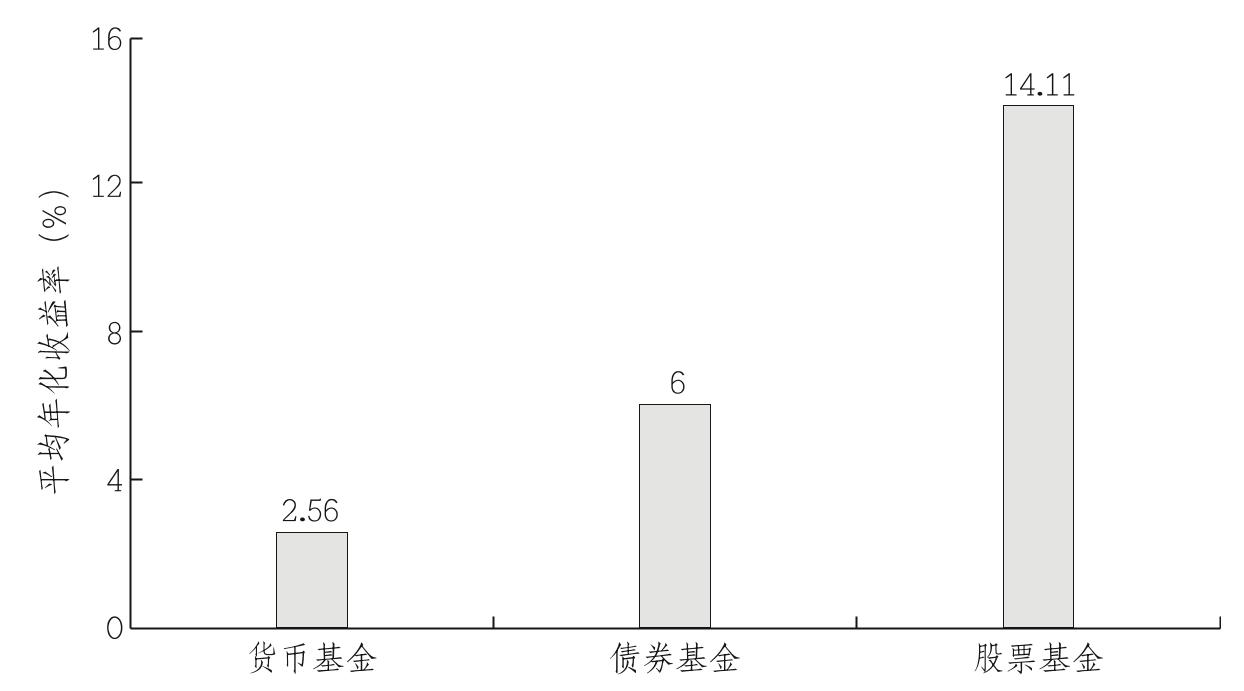
\includegraphics[width=\textwidth,height=0.82\textheight,keepaspectratio]{figure/图4.1.png}
\caption{2004—2017年，我国所有货币基金、债券基金、股票基金的平均年化收益率}\label{fig:4-1}
\end{figure}

从货币基金到债券基金，再到股票基金，它们的年化收益率一个比一个高。长期收益率最高的股票基金，可以帮助我们抵御通货膨胀的侵蚀。

这个特征，跟美国市场这三类资产的特征也是吻合的。

不过，我们投资的时候，不能只看收益情况，还得看投资中要面对的风险。这里的风险，说的主要是持有过程中的波动风险。

虽然从长期来看这三类资产的收益都是上涨的，但是在持有过程中，可能短期会有波动，导致基金的收益出现下跌。

回顾国内这三类基金十几年的收益历史，如图 \ref{fig:4-2} 所示，我们会发现，货币基金从整体来看，几乎没有下跌。它本身波动风险很小，几乎每天都是上涨的。所以货币基金适合用来打理短期不用的零钱，随取所用，也不用太担心风险。

\begin{figure}[htbp]
\centering
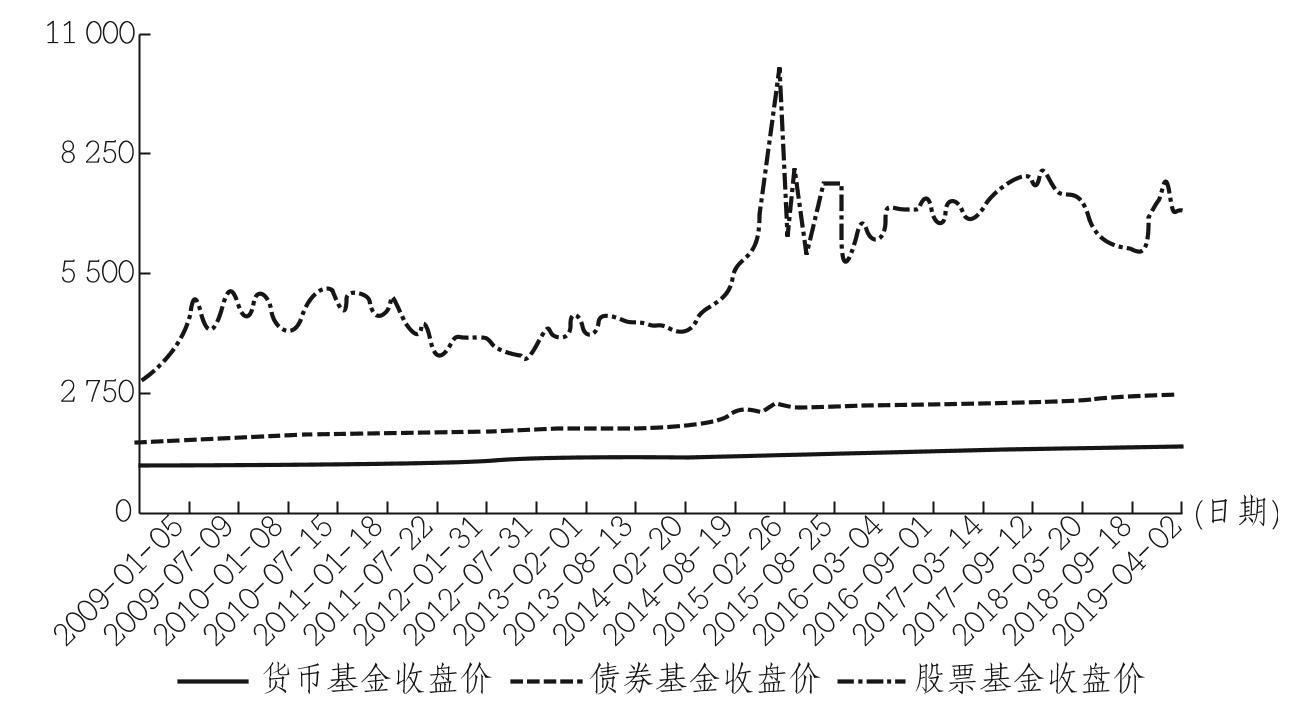
\includegraphics[width=\textwidth,height=0.82\textheight,keepaspectratio]{figure/图4.2.png}
\caption{货币基金、债券基金、股票基金的收盘价}\label{fig:4-2}
\end{figure}

债券基金长期收益比货币基金高，但是它有波动风险。债券基金在持有过程中，可能会出现百分之十几的波动。也就是说，在最差的情况下，可能会短期有百分之十几的浮亏。不过随着投资时间拉长，债券基金也是可以赢利的。

而股票基金的长期收益是这三类基金中最高的，但是波动风险也是这三类基金中最高的。股票基金在持有过程中，可能会出现高达50\%的波动风险。如果投资者不懂得股票基金的投资技巧，可能会出现超过50\%的浮亏。高风险、高收益，是股票基金的特点。

但是长期看，能帮助我们抵抗通货膨胀的，也是股票基金。

所以，我们做定投的操作，把人力资产定期转换为金融资产，里面必须要有一部分是配置到股票资产上。而股票基金，就是很好的定投工具。

但是股票基金的品种非常多，哪一种适合作为我们定投的主力呢？

\subsection{指数基金，定投的主力}
在股票基金中，有两类区别很大的投资品种。一类是主动型股票基金，一类是被动型股票基金。

这里的主动和被动，主要是指基金经理是否主动参与股票的选股和买卖决策。

如果一只股票基金，是基金经理来选择股票，并且决定股票的买入卖出，这种类型的股票基金是主动基金。投资收益取决于基金经理的投资能力。

如果一只股票基金，其基金经理不参与选股，而是根据某一个既定的规则来挑选股票、买入卖出，这种类型的股票基金是被动基金。被动基金的典型代表，就是指数基金。

指数基金是参考指数来挑选股票、买入卖出的。指数本身有事先制定好的选股规则。

简单来说，买主动基金，就是挑人。看好并认可某位基金经理的投资能力，投资其管理的产品。这位基金经理如果跳槽或者更换了自己的产品，通常投资者也会追随他，更换为他管理的基金产品。而买指数基金，则是挑指数。看好并认可某个指数的投资价值。

在定投的时候，我们该选择哪一类股票基金入手呢？

当然是指数基金了。

\subsubsection{巴菲特为什么建议普通投资者投资指数基金}

我们可以听一下“股神”巴菲特的意见。

巴菲特是著名的投资大师，个人资产长期排名在全球富豪榜前几位。巴菲特从学徒起家，在几十年里获取了上万倍的资产增值。

有非常多的人向巴菲特请教投资秘诀，但巴菲特在公开场合只推荐过一个品种：指数基金。

事实上，巴菲特几乎每年都会向普通投资者推荐指数基金。

早在1993年，巴菲特就第一次推荐指数基金。

{\kaishu 通过定投指数基金，一个什么都不懂的业余投资者，往往能够战胜大部分专业投资者。}

到2007年，巴菲特再次推荐指数基金。

{\kaishu 对于绝大多数没有时间进行充分个股调研的中小投资者，成本低廉的指数基金或许是他们投资股市的最佳选择。}

也是在2007年，巴菲特还发起了一个著名的赌局：由对冲基金的基金经理挑选主动基金组合，自己挑选标普500指数基金，看未来10年哪个收益更高。

到2016年年底，标普500指数基金的年复合收益率为7.1\%，同期由基金经理挑选的基金组合的收益率只有2.2\%。很明显，在10年赌约到期之前，巴菲特就赢得了这个赌局。

在对赌开始之前，巴菲特就知道自己必赢无疑。他说：

{\kaishu 我经常推荐的就是低成本的标普500指数基金，但是只有极少数谦虚的朋友才会相信我的话。}

2014年的时候，巴菲特还立下遗嘱：

{\kaishu 如果我过世，我名下90\%的现金将让托管人购买指数基金。}

为什么巴菲特这么推崇指数基金呢？

\subsubsection{指数基金的三大好处}

巴菲特如此青睐指数基金，它一定有过人之处。实际上，指数基金有三大优势，还可以规避三大风险。

第一大优势，指数基金能够长生不老。

举个例子，美国最知名的指数之一是道琼斯指数，它诞生于100多年前。最初道琼斯指数有20只成份股，从100点起步。结果100多年过去了，道琼斯指数从100点慢慢涨到了今天的两万多点。而最初的20只成份股背后的公司一家家衰落，并有新的公司被替换进来。到今天，唯一存活的只有一家通用电气。

因为没有一家公司可以长生不老，但是指数基金可以通过吸收新公司、替换老公司的方法，长生不老。理论上指数的寿命与国家政府的寿命等同。这种新陈代谢带来的永续能力，是个股不具备的。

第二大优势，能够长期上涨。

比如说，道琼斯指数从最初的100点上涨到了现在的两万多点。我们平时总说中国股市不好，但实际上中国股市的平均收益是非常不错的。衡量上海证券交易所平均股价的上证综指，从1991年年初的100点，上涨到了今天的2000多点，年化收益率也达到了15\%左右。

巴菲特也提到，买指数基金就是买国运。只要相信国家能继续发展，指数基金就能长期上涨，我们就能分享国家经济增长的收益。

第三大优势，费用低廉。

每一只基金都会收取基金管理费和托管费，这是基金公司重要的收入来源，每一只基金都会有这些费用。这些费用是在后台收取的，我们并不能直接看到，但每年都会收取一次。不同的基金管理费和托管费并不一样。

像指数基金，一般会收取每年0.6\%～0.8\%的费率，而普通的股票基金，会收取1.2\%～2\%的费率。这个意味着什么呢？假如我们买1万元的指数基金，一年要交60～80元的费用；如果买1万元的普通股票基金，一年要交120～200元的费用。长期下来，差距还是很大的。

\subsubsection{指数基金可以避免三大类风险}

另外，相比于一般的股票和股票基金，指数基金可以避免三大类风险。

第一类风险，是个股“黑天鹅”风险。像这种无法预料的风险，在指数基金中几乎不会出现。因为指数基金包括几十甚至上百只股票，单只股票出现问题并没有多少影响。而且，指数基金还会根据公司的经营情况及时调整，去除经营不好的公司，换进经营好的公司，进一步减少了这种无法预料的风险。

第二类风险，是本金永久损失的风险。个股可能会遇到企业经营上的问题，导致个股破产倒闭，投资者血本无归。但指数基金即使下跌也会有限度，不会跌没。这种特性帮我们规避了本金永久损失的风险。

第三类风险，是制度风险。指数基金是按照指数来选股，而指数的规则是早就确立好了的，任何人都可以查询、监督。所以指数基金不会有“老鼠仓”、利益输送等情况出现。

关于指数基金的好处，以及更详细、更深入的知识，大家可以通过阅读《指数基金投资指南》这本书获得。

\subsubsection{投资者笔记}

\begin{itemize}
\item {\kaishu 基金，是最适合普通投资者的工具。}
\item {\kaishu 按照投资方向，基金可以分为：股票基金、债券基金、混合基金、货币基金。其中能帮助我们抵御通货膨胀的，主要是股票基金。}
\item {\kaishu 股票基金中，最适合普通投资者的是指数基金。}
\item {\kaishu 指数基金有三个独特的好处：长生不老，长期上涨，费率低廉，因此它是我们定投的主力。}
\end{itemize}

